\chapter{Validation software}

It was important to validate the calculations done in this project continuously. As many of the calculations are not static, but because of inertial forces is was important visualize these changes as they were happening. It was decided that implementing this feature in GeoMod would be too time consuming because of it's size and complexity. 

It was therefore necessary to create a smaller program that would be able to do the calculations and visualize the results. That way, the algorithms could be validated and their practicality determined as fast as possible. This approach can be compared to rapid prototyping in traditional manufacturing, fail early to succeed sooner.


\section{Interface}

\figref{interface} shows the interface for the completed software created in QtCreator. This section will give a short overview of the functionality of the software, starting with the left column.

\textsf{Add links} lets the user define a revolute manipulator arm by the \gls{DH} or \textsf{Add default links} can be used to insert a predefined manipulator. By selecting a specific link in the list, it's variables can be viewed and changed in the \textsf{Weight} and \textsf{Joint angle} section. A start and end angle can be defined for each link with the \textsf{Set start/end} button. By pressing the \textsf{to start/end} button the whole manipulator will animate between these configurations over a time specified as in \textsf{Animation time}. The \textsf{Print robot} button will print the transformation matrix for each link and the robot as a whole to the console as in \figref{console}.

\begin{figure}[h!]
    \centering
    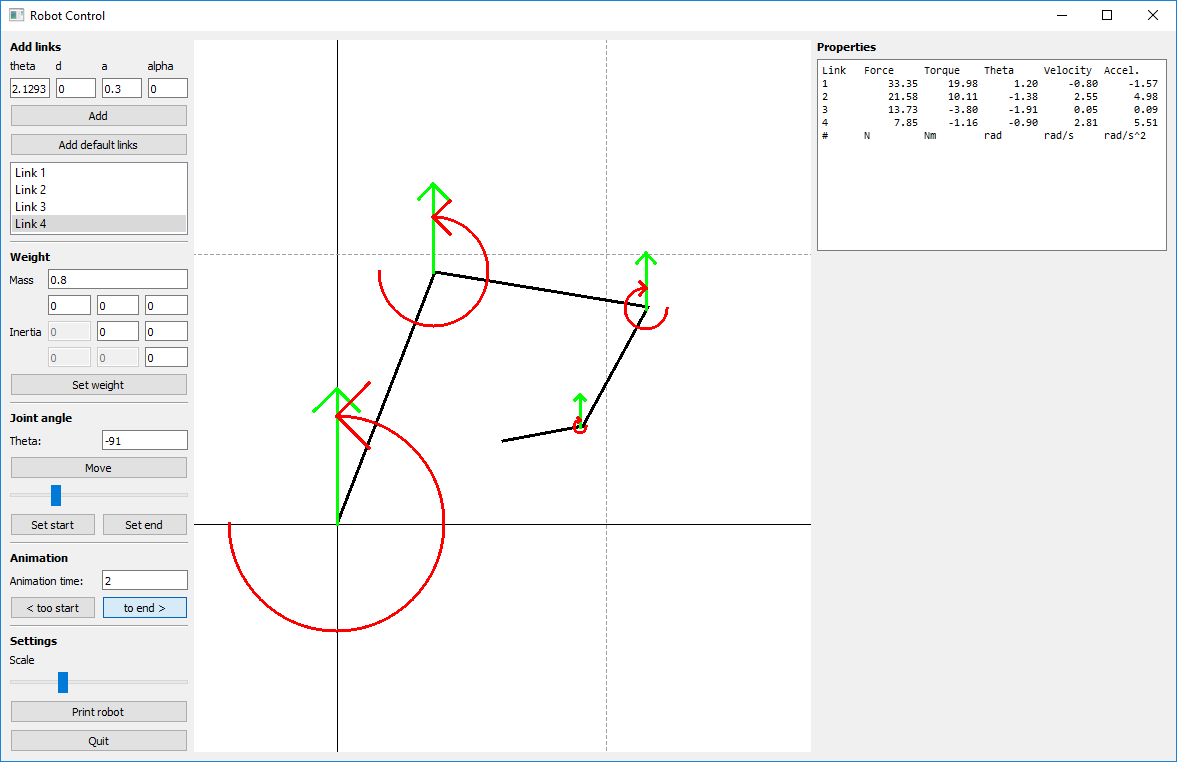
\includegraphics[width=\textwidth]{robot_control_interface2}
    \caption{Main interface of \textit{Robot Control} validation software}
    \label{interface}
\end{figure}

The central area shows the robot and the joint forces and torques in green and red respectively. The larger the arrow, the larger the force or torque is. Graphics can be panned and zoomed with the middle mouse button. Lastly, the right hand side shows useful information for each link and are updated continuously. These are helpful properties used for debugging and validation.

\begin{figure}[h!]
    \centering
    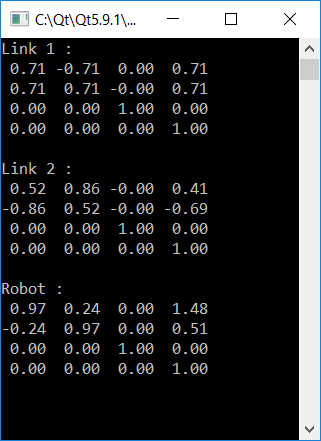
\includegraphics[width=.4\textwidth]{robot_control_console}
    \caption{Printed transformation matrices, here for a two-armed manipulator.}
    \label{console}
\end{figure}

\section{Class overview}

This section will give a short overview of the most important classes and properties relevant for the dynamic calculations.

\todo[inline]{
\textbf{Todo}

- Describe the intention and structure of the following classes:

- Robot, Link, Transformation and RenderArea class
}

\section{Drawing}

\todo[inline]{
\textbf{Todo}

- Describe how the QPainter class works

- Method for drawing arrows

- All the calculations are done for a 3D case, but everything is shown in 2D
}

\section{Animation}

\todo[inline]{
\textbf{Todo}

- It was important to have continuous moving links to verify the calculations

- start and end for each link can be set

- animation between these values, quintic graphs

- computer time is stored for last position so that derivatives can be calculated

- Must be calculated in a way that does not depend on the computer or available processing power, not a fixed frames per second
}